\documentclass[twoside]{book}

% Packages required by doxygen
\usepackage{calc}
\usepackage{doxygen}
\usepackage{graphicx}
\usepackage[utf8]{inputenc}
\usepackage{makeidx}
\usepackage{multicol}
\usepackage{multirow}
\usepackage{fixltx2e}
\PassOptionsToPackage{warn}{textcomp}
\usepackage{textcomp}
\usepackage[nointegrals]{wasysym}
\usepackage[table]{xcolor}

% Font selection
\usepackage[T1]{fontenc}
\usepackage{mathptmx}
\usepackage[scaled=.90]{helvet}
\usepackage{courier}
\usepackage{amssymb}
\usepackage{sectsty}
\renewcommand{\familydefault}{\sfdefault}
\allsectionsfont{%
  \fontseries{bc}\selectfont%
  \color{darkgray}%
}
\renewcommand{\DoxyLabelFont}{%
  \fontseries{bc}\selectfont%
  \color{darkgray}%
}
\newcommand{\+}{\discretionary{\mbox{\scriptsize$\hookleftarrow$}}{}{}}

% Page & text layout
\usepackage{geometry}
\geometry{%
  a4paper,%
  top=2.5cm,%
  bottom=2.5cm,%
  left=2.5cm,%
  right=2.5cm%
}
\tolerance=750
\hfuzz=15pt
\hbadness=750
\setlength{\emergencystretch}{15pt}
\setlength{\parindent}{0cm}
\setlength{\parskip}{0.2cm}
\makeatletter
\renewcommand{\paragraph}{%
  \@startsection{paragraph}{4}{0ex}{-1.0ex}{1.0ex}{%
    \normalfont\normalsize\bfseries\SS@parafont%
  }%
}
\renewcommand{\subparagraph}{%
  \@startsection{subparagraph}{5}{0ex}{-1.0ex}{1.0ex}{%
    \normalfont\normalsize\bfseries\SS@subparafont%
  }%
}
\makeatother

% Headers & footers
\usepackage{fancyhdr}
\pagestyle{fancyplain}
\fancyhead[LE]{\fancyplain{}{\bfseries\thepage}}
\fancyhead[CE]{\fancyplain{}{}}
\fancyhead[RE]{\fancyplain{}{\bfseries\leftmark}}
\fancyhead[LO]{\fancyplain{}{\bfseries\rightmark}}
\fancyhead[CO]{\fancyplain{}{}}
\fancyhead[RO]{\fancyplain{}{\bfseries\thepage}}
\fancyfoot[LE]{\fancyplain{}{}}
\fancyfoot[CE]{\fancyplain{}{}}
\fancyfoot[RE]{\fancyplain{}{\bfseries\scriptsize Generated on Fri May 16 2014 14\+:37\+:09 for Legos by Doxygen }}
\fancyfoot[LO]{\fancyplain{}{\bfseries\scriptsize Generated on Fri May 16 2014 14\+:37\+:09 for Legos by Doxygen }}
\fancyfoot[CO]{\fancyplain{}{}}
\fancyfoot[RO]{\fancyplain{}{}}
\renewcommand{\footrulewidth}{0.4pt}
\renewcommand{\chaptermark}[1]{%
  \markboth{#1}{}%
}
\renewcommand{\sectionmark}[1]{%
  \markright{\thesection\ #1}%
}

% Indices & bibliography
\usepackage{natbib}
\usepackage[titles]{tocloft}
\setcounter{tocdepth}{3}
\setcounter{secnumdepth}{5}
\makeindex

% Hyperlinks (required, but should be loaded last)
\usepackage{ifpdf}
\ifpdf
  \usepackage[pdftex,pagebackref=true]{hyperref}
\else
  \usepackage[ps2pdf,pagebackref=true]{hyperref}
\fi
\hypersetup{%
  colorlinks=true,%
  linkcolor=blue,%
  citecolor=blue,%
  unicode%
}

% Custom commands
\newcommand{\clearemptydoublepage}{%
  \newpage{\pagestyle{empty}\cleardoublepage}%
}


%===== C O N T E N T S =====

\begin{document}

% Titlepage & ToC
\hypersetup{pageanchor=false,
             bookmarks=true,
             bookmarksnumbered=true,
             pdfencoding=unicode
            }
\pagenumbering{roman}
\begin{titlepage}
\vspace*{7cm}
\begin{center}%
{\Large Legos }\\
\vspace*{1cm}
{\large Generated by Doxygen 1.8.7}\\
\vspace*{0.5cm}
{\small Fri May 16 2014 14:37:09}\\
\end{center}
\end{titlepage}
\clearemptydoublepage
\tableofcontents
\clearemptydoublepage
\pagenumbering{arabic}
\hypersetup{pageanchor=true}

%--- Begin generated contents ---
\chapter{Namespace Index}
\section{Packages}
Here are the packages with brief descriptions (if available)\+:\begin{DoxyCompactList}
\item\contentsline{section}{\hyperlink{namespace_gene}{Gene} \\*This class is responsible for managing a gene object }{\pageref{namespace_gene}}{}
\item\contentsline{section}{\hyperlink{namespace_gene_test}{Gene\+Test} \\*This class is responsible for unit testing the gene class }{\pageref{namespace_gene_test}}{}
\end{DoxyCompactList}

\chapter{Hierarchical Index}
\section{Class Hierarchy}
This inheritance list is sorted roughly, but not completely, alphabetically\+:\begin{DoxyCompactList}
\item \contentsline{section}{gene.\+Gene}{\pageref{classgene_1_1_gene}}{}
\item Test\+Case\begin{DoxyCompactList}
\item \contentsline{section}{gene.\+Gene\+Test}{\pageref{classgene_1_1_gene_test}}{}
\end{DoxyCompactList}
\end{DoxyCompactList}

\chapter{Class Index}
\section{Class List}
Here are the classes, structs, unions and interfaces with brief descriptions\+:\begin{DoxyCompactList}
\item\contentsline{section}{\hyperlink{classgene_1_1_gene}{gene.\+Gene} }{\pageref{classgene_1_1_gene}}{}
\item\contentsline{section}{\hyperlink{classgene_1_1_gene_test}{gene.\+Gene\+Test} }{\pageref{classgene_1_1_gene_test}}{}
\end{DoxyCompactList}

\chapter{Namespace Documentation}
\hypertarget{namespace_gene}{\section{Gene Namespace Reference}
\label{namespace_gene}\index{Gene@{Gene}}
}


This class is responsible for managing a gene object.  




\subsection{Detailed Description}
This class is responsible for managing a gene object. 
\hypertarget{namespace_gene_test}{\section{Gene\+Test Namespace Reference}
\label{namespace_gene_test}\index{Gene\+Test@{Gene\+Test}}
}


This class is responsible for unit testing the gene class.  




\subsection{Detailed Description}
This class is responsible for unit testing the gene class. 
\chapter{Class Documentation}
\hypertarget{classgene_1_1_gene}{\section{gene.\+Gene Class Reference}
\label{classgene_1_1_gene}\index{gene.\+Gene@{gene.\+Gene}}
}
\subsection*{Public Member Functions}
\begin{DoxyCompactItemize}
\item 
def \hyperlink{classgene_1_1_gene_a83b42158e952b57f232670532e64246c}{\+\_\+\+\_\+init\+\_\+\+\_\+}
\begin{DoxyCompactList}\small\item\em The constructor. \end{DoxyCompactList}\item 
def \hyperlink{classgene_1_1_gene_a022015d0044621d4a0f23f877ecdf41f}{add\+Transcript\+I\+D}
\begin{DoxyCompactList}\small\item\em Add a transcript I\+D. \end{DoxyCompactList}\item 
def \hyperlink{classgene_1_1_gene_a395bb5c95232ee0acabd23487b2e5eac}{get\+Name}
\begin{DoxyCompactList}\small\item\em Get the name of the gene. \end{DoxyCompactList}\item 
def \hyperlink{classgene_1_1_gene_a26bf7de0fc7c79c3716f8514401e4ba0}{get\+Transcript\+I\+D}
\begin{DoxyCompactList}\small\item\em Get the transcript I\+D. \end{DoxyCompactList}\item 
def \hyperlink{classgene_1_1_gene_a5c75d7129fb82095e60697a6ada6af4e}{get\+Chromosome}
\begin{DoxyCompactList}\small\item\em Get the chromosome. \end{DoxyCompactList}\item 
def \hyperlink{classgene_1_1_gene_ad5a8abe5ba76e5ce49ef34a2066a4966}{get\+Strand}
\begin{DoxyCompactList}\small\item\em Get the strand. \end{DoxyCompactList}\item 
def \hyperlink{classgene_1_1_gene_aa719d094a9f3cd14d28b09a9f04b90f0}{get\+Start\+Position}
\begin{DoxyCompactList}\small\item\em Get the start position. \end{DoxyCompactList}\item 
def \hyperlink{classgene_1_1_gene_ad2ebf59eeeb3a10a8ad586eaf066554c}{get\+End\+Position}
\begin{DoxyCompactList}\small\item\em Get the end position. \end{DoxyCompactList}\item 
def \hyperlink{classgene_1_1_gene_a4f1b596217ec43b206f9277128b82640}{add\+Exons\+To\+Gene}
\begin{DoxyCompactList}\small\item\em Add exons to the gene. \end{DoxyCompactList}\item 
def \hyperlink{classgene_1_1_gene_a64e9f4b793f36ef68a5b6d837f5d3d07}{get\+Location}
\begin{DoxyCompactList}\small\item\em Given a coordinate position this will return the location of the coordinate (upstream, downstream, exon, or intron) and the distance from the gene. \end{DoxyCompactList}\end{DoxyCompactItemize}
\subsection*{Public Attributes}
\begin{DoxyCompactItemize}
\item 
\hypertarget{classgene_1_1_gene_a759b35e75288028984867d2d81a623c0}{{\bfseries name}}\label{classgene_1_1_gene_a759b35e75288028984867d2d81a623c0}

\item 
\hypertarget{classgene_1_1_gene_a4c2abcb3266331ffeb5613fc462d29bc}{{\bfseries chromosome}}\label{classgene_1_1_gene_a4c2abcb3266331ffeb5613fc462d29bc}

\item 
\hypertarget{classgene_1_1_gene_aa6c5425d595f6fe6eef36c4d9051465a}{{\bfseries strand}}\label{classgene_1_1_gene_aa6c5425d595f6fe6eef36c4d9051465a}

\item 
\hypertarget{classgene_1_1_gene_a5a6135b9254abcb4fff6a5a33a106e40}{{\bfseries start\+Position}}\label{classgene_1_1_gene_a5a6135b9254abcb4fff6a5a33a106e40}

\item 
\hypertarget{classgene_1_1_gene_a950fbd02d87d8bb0ae8ffb97c595e541}{{\bfseries end\+Position}}\label{classgene_1_1_gene_a950fbd02d87d8bb0ae8ffb97c595e541}

\item 
\hypertarget{classgene_1_1_gene_a3f675c67c0eec4dc6b139f7fce064f16}{{\bfseries exon\+Starts}}\label{classgene_1_1_gene_a3f675c67c0eec4dc6b139f7fce064f16}

\item 
\hypertarget{classgene_1_1_gene_a9d48a8038f178a63f3e9e78fae2b789d}{{\bfseries exon\+Ends}}\label{classgene_1_1_gene_a9d48a8038f178a63f3e9e78fae2b789d}

\item 
\hypertarget{classgene_1_1_gene_a5056318fb7e1d83a2cc92fd824fe8ee7}{{\bfseries sequence}}\label{classgene_1_1_gene_a5056318fb7e1d83a2cc92fd824fe8ee7}

\item 
\hypertarget{classgene_1_1_gene_ab8cd030ea42614d353ad58c07bbdd85f}{{\bfseries transcript\+I\+D}}\label{classgene_1_1_gene_ab8cd030ea42614d353ad58c07bbdd85f}

\end{DoxyCompactItemize}
\subsection*{Static Public Attributes}
\begin{DoxyCompactItemize}
\item 
\hypertarget{classgene_1_1_gene_a708074195322ffe28b19ec04eb703646}{string {\bfseries name} = \char`\"{}\char`\"{}}\label{classgene_1_1_gene_a708074195322ffe28b19ec04eb703646}

\item 
\hypertarget{classgene_1_1_gene_a453e9df0d07b23f6ade41ae635ca003c}{string {\bfseries transcript\+I\+D} = \char`\"{}\char`\"{}}\label{classgene_1_1_gene_a453e9df0d07b23f6ade41ae635ca003c}

\item 
\hypertarget{classgene_1_1_gene_adf9c516959efc5d643eb7de01e50a04b}{string {\bfseries chromosome} = \char`\"{}\char`\"{}}\label{classgene_1_1_gene_adf9c516959efc5d643eb7de01e50a04b}

\item 
\hypertarget{classgene_1_1_gene_a4f33daaa0bde33b9c0ce44cbcc03f82f}{string {\bfseries strand} = \char`\"{}\char`\"{}}\label{classgene_1_1_gene_a4f33daaa0bde33b9c0ce44cbcc03f82f}

\item 
\hypertarget{classgene_1_1_gene_a51139d8882bb9fed480504dd6aef712e}{int {\bfseries start\+Position} = 0}\label{classgene_1_1_gene_a51139d8882bb9fed480504dd6aef712e}

\item 
\hypertarget{classgene_1_1_gene_a57c01bf45d3dcbe94ead6f7f999ee719}{int {\bfseries end\+Position} = 0}\label{classgene_1_1_gene_a57c01bf45d3dcbe94ead6f7f999ee719}

\item 
\hypertarget{classgene_1_1_gene_a5f4fc7068e32531eef0fc2ab8faaaea8}{list {\bfseries exon\+Starts} = \mbox{[}$\,$\mbox{]}}\label{classgene_1_1_gene_a5f4fc7068e32531eef0fc2ab8faaaea8}

\item 
\hypertarget{classgene_1_1_gene_adcf9f27e981a5db63976f95015fffe47}{list {\bfseries exon\+Ends} = \mbox{[}$\,$\mbox{]}}\label{classgene_1_1_gene_adcf9f27e981a5db63976f95015fffe47}

\item 
\hypertarget{classgene_1_1_gene_af3db36708f8deb872b4d0391ef663df9}{string {\bfseries sequence} = \char`\"{}\char`\"{}}\label{classgene_1_1_gene_af3db36708f8deb872b4d0391ef663df9}

\end{DoxyCompactItemize}


\subsection{Constructor \& Destructor Documentation}
\hypertarget{classgene_1_1_gene_a83b42158e952b57f232670532e64246c}{\index{gene\+::\+Gene@{gene\+::\+Gene}!\+\_\+\+\_\+init\+\_\+\+\_\+@{\+\_\+\+\_\+init\+\_\+\+\_\+}}
\index{\+\_\+\+\_\+init\+\_\+\+\_\+@{\+\_\+\+\_\+init\+\_\+\+\_\+}!gene\+::\+Gene@{gene\+::\+Gene}}
\subsubsection[{\+\_\+\+\_\+init\+\_\+\+\_\+}]{\setlength{\rightskip}{0pt plus 5cm}def gene.\+Gene.\+\_\+\+\_\+init\+\_\+\+\_\+ (
\begin{DoxyParamCaption}
\item[{}]{self, }
\item[{}]{name, }
\item[{}]{chromosome, }
\item[{}]{strand, }
\item[{}]{start\+Position, }
\item[{}]{end\+Position}
\end{DoxyParamCaption}
)}}\label{classgene_1_1_gene_a83b42158e952b57f232670532e64246c}


The constructor. 


\begin{DoxyParams}{Parameters}
{\em self} & The object pointer \\
\hline
{\em name} & The name of the gene \\
\hline
{\em chromosome} & The name of the chromosome (e.\+g. chr1) \\
\hline
{\em strand} & The strand of the gene (e.\+g. F or R) \\
\hline
{\em start\+Position} & The start position \\
\hline
{\em end\+Position} & The end position \\
\hline
\end{DoxyParams}


\subsection{Member Function Documentation}
\hypertarget{classgene_1_1_gene_a4f1b596217ec43b206f9277128b82640}{\index{gene\+::\+Gene@{gene\+::\+Gene}!add\+Exons\+To\+Gene@{add\+Exons\+To\+Gene}}
\index{add\+Exons\+To\+Gene@{add\+Exons\+To\+Gene}!gene\+::\+Gene@{gene\+::\+Gene}}
\subsubsection[{add\+Exons\+To\+Gene}]{\setlength{\rightskip}{0pt plus 5cm}def gene.\+Gene.\+add\+Exons\+To\+Gene (
\begin{DoxyParamCaption}
\item[{}]{self, }
\item[{}]{starts, }
\item[{}]{ends}
\end{DoxyParamCaption}
)}}\label{classgene_1_1_gene_a4f1b596217ec43b206f9277128b82640}


Add exons to the gene. 


\begin{DoxyParams}{Parameters}
{\em self} & The object pointer \\
\hline
{\em starts} & A comma-\/separated string of start coordinates \\
\hline
{\em ends} & A comma-\/separated string of end coordinates \\
\hline
\end{DoxyParams}
\hypertarget{classgene_1_1_gene_a022015d0044621d4a0f23f877ecdf41f}{\index{gene\+::\+Gene@{gene\+::\+Gene}!add\+Transcript\+I\+D@{add\+Transcript\+I\+D}}
\index{add\+Transcript\+I\+D@{add\+Transcript\+I\+D}!gene\+::\+Gene@{gene\+::\+Gene}}
\subsubsection[{add\+Transcript\+I\+D}]{\setlength{\rightskip}{0pt plus 5cm}def gene.\+Gene.\+add\+Transcript\+I\+D (
\begin{DoxyParamCaption}
\item[{}]{self, }
\item[{}]{transcript\+I\+D}
\end{DoxyParamCaption}
)}}\label{classgene_1_1_gene_a022015d0044621d4a0f23f877ecdf41f}


Add a transcript I\+D. 


\begin{DoxyParams}{Parameters}
{\em self} & The object pointer \\
\hline
{\em transcript\+I\+D} & The transcript I\+D \\
\hline
\end{DoxyParams}
\hypertarget{classgene_1_1_gene_a5c75d7129fb82095e60697a6ada6af4e}{\index{gene\+::\+Gene@{gene\+::\+Gene}!get\+Chromosome@{get\+Chromosome}}
\index{get\+Chromosome@{get\+Chromosome}!gene\+::\+Gene@{gene\+::\+Gene}}
\subsubsection[{get\+Chromosome}]{\setlength{\rightskip}{0pt plus 5cm}def gene.\+Gene.\+get\+Chromosome (
\begin{DoxyParamCaption}
\item[{}]{self}
\end{DoxyParamCaption}
)}}\label{classgene_1_1_gene_a5c75d7129fb82095e60697a6ada6af4e}


Get the chromosome. 


\begin{DoxyParams}{Parameters}
{\em self} & The object pointer \\
\hline
\end{DoxyParams}
\begin{DoxyReturn}{Returns}
Returns the chromosome of the gene 
\end{DoxyReturn}
\hypertarget{classgene_1_1_gene_ad2ebf59eeeb3a10a8ad586eaf066554c}{\index{gene\+::\+Gene@{gene\+::\+Gene}!get\+End\+Position@{get\+End\+Position}}
\index{get\+End\+Position@{get\+End\+Position}!gene\+::\+Gene@{gene\+::\+Gene}}
\subsubsection[{get\+End\+Position}]{\setlength{\rightskip}{0pt plus 5cm}def gene.\+Gene.\+get\+End\+Position (
\begin{DoxyParamCaption}
\item[{}]{self}
\end{DoxyParamCaption}
)}}\label{classgene_1_1_gene_ad2ebf59eeeb3a10a8ad586eaf066554c}


Get the end position. 


\begin{DoxyParams}{Parameters}
{\em self} & The object pointer \\
\hline
\end{DoxyParams}
\begin{DoxyReturn}{Returns}
Returns the end position of the gene 
\end{DoxyReturn}
\hypertarget{classgene_1_1_gene_a64e9f4b793f36ef68a5b6d837f5d3d07}{\index{gene\+::\+Gene@{gene\+::\+Gene}!get\+Location@{get\+Location}}
\index{get\+Location@{get\+Location}!gene\+::\+Gene@{gene\+::\+Gene}}
\subsubsection[{get\+Location}]{\setlength{\rightskip}{0pt plus 5cm}def gene.\+Gene.\+get\+Location (
\begin{DoxyParamCaption}
\item[{}]{self, }
\item[{}]{position}
\end{DoxyParamCaption}
)}}\label{classgene_1_1_gene_a64e9f4b793f36ef68a5b6d837f5d3d07}


Given a coordinate position this will return the location of the coordinate (upstream, downstream, exon, or intron) and the distance from the gene. 

If the coordinate is in the gene then it will return the exon or intron number 
\begin{DoxyParams}{Parameters}
{\em self} & The object pointer \\
\hline
{\em position} & The position to test \\
\hline
\end{DoxyParams}
\begin{DoxyReturn}{Returns}
Returns the location of the intron (upstream, downstream, exon, intron) and the distance from the gene or exon / intron number if within gene 
\end{DoxyReturn}
\hypertarget{classgene_1_1_gene_a395bb5c95232ee0acabd23487b2e5eac}{\index{gene\+::\+Gene@{gene\+::\+Gene}!get\+Name@{get\+Name}}
\index{get\+Name@{get\+Name}!gene\+::\+Gene@{gene\+::\+Gene}}
\subsubsection[{get\+Name}]{\setlength{\rightskip}{0pt plus 5cm}def gene.\+Gene.\+get\+Name (
\begin{DoxyParamCaption}
\item[{}]{self}
\end{DoxyParamCaption}
)}}\label{classgene_1_1_gene_a395bb5c95232ee0acabd23487b2e5eac}


Get the name of the gene. 


\begin{DoxyParams}{Parameters}
{\em self} & The object pointer \\
\hline
\end{DoxyParams}
\begin{DoxyReturn}{Returns}
Returns the name of the gene 
\end{DoxyReturn}
\hypertarget{classgene_1_1_gene_aa719d094a9f3cd14d28b09a9f04b90f0}{\index{gene\+::\+Gene@{gene\+::\+Gene}!get\+Start\+Position@{get\+Start\+Position}}
\index{get\+Start\+Position@{get\+Start\+Position}!gene\+::\+Gene@{gene\+::\+Gene}}
\subsubsection[{get\+Start\+Position}]{\setlength{\rightskip}{0pt plus 5cm}def gene.\+Gene.\+get\+Start\+Position (
\begin{DoxyParamCaption}
\item[{}]{self}
\end{DoxyParamCaption}
)}}\label{classgene_1_1_gene_aa719d094a9f3cd14d28b09a9f04b90f0}


Get the start position. 


\begin{DoxyParams}{Parameters}
{\em self} & The object pointer \\
\hline
\end{DoxyParams}
\begin{DoxyReturn}{Returns}
Returns the start position of the gene 
\end{DoxyReturn}
\hypertarget{classgene_1_1_gene_ad5a8abe5ba76e5ce49ef34a2066a4966}{\index{gene\+::\+Gene@{gene\+::\+Gene}!get\+Strand@{get\+Strand}}
\index{get\+Strand@{get\+Strand}!gene\+::\+Gene@{gene\+::\+Gene}}
\subsubsection[{get\+Strand}]{\setlength{\rightskip}{0pt plus 5cm}def gene.\+Gene.\+get\+Strand (
\begin{DoxyParamCaption}
\item[{}]{self}
\end{DoxyParamCaption}
)}}\label{classgene_1_1_gene_ad5a8abe5ba76e5ce49ef34a2066a4966}


Get the strand. 


\begin{DoxyParams}{Parameters}
{\em self} & The object pointer \\
\hline
\end{DoxyParams}
\begin{DoxyReturn}{Returns}
Returns the strand of the gene 
\end{DoxyReturn}
\hypertarget{classgene_1_1_gene_a26bf7de0fc7c79c3716f8514401e4ba0}{\index{gene\+::\+Gene@{gene\+::\+Gene}!get\+Transcript\+I\+D@{get\+Transcript\+I\+D}}
\index{get\+Transcript\+I\+D@{get\+Transcript\+I\+D}!gene\+::\+Gene@{gene\+::\+Gene}}
\subsubsection[{get\+Transcript\+I\+D}]{\setlength{\rightskip}{0pt plus 5cm}def gene.\+Gene.\+get\+Transcript\+I\+D (
\begin{DoxyParamCaption}
\item[{}]{self}
\end{DoxyParamCaption}
)}}\label{classgene_1_1_gene_a26bf7de0fc7c79c3716f8514401e4ba0}


Get the transcript I\+D. 


\begin{DoxyParams}{Parameters}
{\em self} & The object pointer \\
\hline
\end{DoxyParams}
\begin{DoxyReturn}{Returns}
Returns the transcript I\+D of the gene 
\end{DoxyReturn}


The documentation for this class was generated from the following file\+:\begin{DoxyCompactItemize}
\item 
bio/gene/gene.\+py\end{DoxyCompactItemize}

\hypertarget{classgene_1_1_gene_test}{\section{gene.\+Gene\+Test Class Reference}
\label{classgene_1_1_gene_test}\index{gene.\+Gene\+Test@{gene.\+Gene\+Test}}
}
Inheritance diagram for gene.\+Gene\+Test\+:\begin{figure}[H]
\begin{center}
\leavevmode
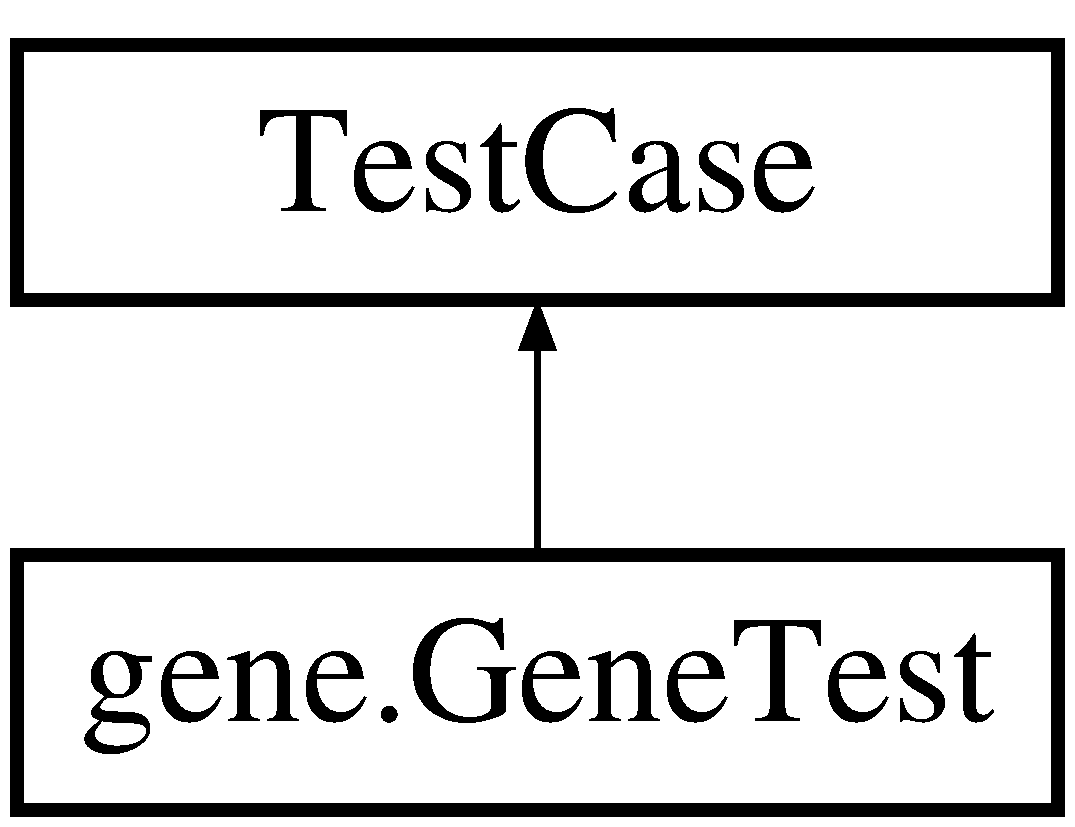
\includegraphics[height=2.000000cm]{classgene_1_1_gene_test}
\end{center}
\end{figure}
\subsection*{Public Member Functions}
\begin{DoxyCompactItemize}
\item 
\hypertarget{classgene_1_1_gene_test_a8748a3d66c9c09a533df5932a79c5cf1}{def {\bfseries test\+\_\+location\+\_\+exon\+\_\+forward}}\label{classgene_1_1_gene_test_a8748a3d66c9c09a533df5932a79c5cf1}

\item 
\hypertarget{classgene_1_1_gene_test_a8c90d274635f61e50aad2f591b966ce7}{def {\bfseries test\+\_\+location\+\_\+intron\+\_\+forward}}\label{classgene_1_1_gene_test_a8c90d274635f61e50aad2f591b966ce7}

\item 
\hypertarget{classgene_1_1_gene_test_a3d7f2c883084688cf189d2164c45d1ef}{def {\bfseries test\+\_\+location\+\_\+upstream\+\_\+forward}}\label{classgene_1_1_gene_test_a3d7f2c883084688cf189d2164c45d1ef}

\item 
\hypertarget{classgene_1_1_gene_test_a770d7f020115c7fbf672b202777799a7}{def {\bfseries test\+\_\+location\+\_\+downstream\+\_\+forward}}\label{classgene_1_1_gene_test_a770d7f020115c7fbf672b202777799a7}

\item 
\hypertarget{classgene_1_1_gene_test_ab802589cf72702568db73d204175d51d}{def {\bfseries test\+\_\+location\+\_\+exon\+\_\+reverse}}\label{classgene_1_1_gene_test_ab802589cf72702568db73d204175d51d}

\item 
\hypertarget{classgene_1_1_gene_test_a82df44ffd0b6b0a929c5aea1e2357958}{def {\bfseries test\+\_\+location\+\_\+intron\+\_\+reverse}}\label{classgene_1_1_gene_test_a82df44ffd0b6b0a929c5aea1e2357958}

\item 
\hypertarget{classgene_1_1_gene_test_a19cf63df4ca1cc366a26174dcd0ad11e}{def {\bfseries test\+\_\+location\+\_\+upstream\+\_\+reverse}}\label{classgene_1_1_gene_test_a19cf63df4ca1cc366a26174dcd0ad11e}

\item 
\hypertarget{classgene_1_1_gene_test_a882d809591797ca533e96f6bb85f5ce6}{def {\bfseries test\+\_\+location\+\_\+downstream\+\_\+reverse}}\label{classgene_1_1_gene_test_a882d809591797ca533e96f6bb85f5ce6}

\end{DoxyCompactItemize}
\subsection*{Static Public Attributes}
\begin{DoxyCompactItemize}
\item 
\hypertarget{classgene_1_1_gene_test_ae96763b3569f91d16621d96a46664b37}{tuple {\bfseries gene\+Forward} = \hyperlink{classgene_1_1_gene}{Gene}(\char`\"{}test\char`\"{}, \char`\"{}chr1\char`\"{}, \char`\"{}F\char`\"{}, 500, 1000)}\label{classgene_1_1_gene_test_ae96763b3569f91d16621d96a46664b37}

\item 
\hypertarget{classgene_1_1_gene_test_a5167ddb04d3f17a8f6598e7c0566ce38}{tuple {\bfseries gene\+Reverse} = \hyperlink{classgene_1_1_gene}{Gene}(\char`\"{}test\char`\"{}, \char`\"{}chr1\char`\"{}, \char`\"{}R\char`\"{}, 1500, 2000)}\label{classgene_1_1_gene_test_a5167ddb04d3f17a8f6598e7c0566ce38}

\end{DoxyCompactItemize}


The documentation for this class was generated from the following file\+:\begin{DoxyCompactItemize}
\item 
bio/gene/gene.\+py\end{DoxyCompactItemize}

%--- End generated contents ---

% Index
\newpage
\phantomsection
\addcontentsline{toc}{chapter}{Index}
\printindex

\end{document}
